\section{Mean-shift segmentation}

Next we analyze the Mean-shift algorithm. One of its main advantages with
respect to k-means is that we do not get to decide the number of clusters.
Instead there is only one parameter to tweak: the bandwidth, which decides
the size of the neighborhood that is considered to compute the direction
towards which the currently selected active point should move. The number
of clusters is decided for each image depending on the data and on the
bandwidth value.
This makes it quite more adaptable to different images. However its main
disadvantage became apparent when performing the experiments for this
section: it is notably slower than k-means because it starts with as many
active points as pixels there are in the image. For the purpose of our
experiments we have found that a bandwidth of 30 yields good results in
a reasonable amount of time, so this is the employed value in all the
examples (unless stated otherwise).

We can see in figure in figure \ref{fig:animals-d30-no-spatial} that the
segmentation is quite good, segmenting the baby lion almost as a whole.
One inconvenient is that the tigers and part of the primate
are included in the same cluster, which is reasonable given than they have
very similar colors and we are using a segmentation technique that is purely driven
by color information. Another disadvantage is that since we are not including
spatial information, there is low uniformity in the grass section.
However if our purpose is to separate the
foreground from the background, Mean-shift is an effective technique to do so.

\begin{figure}[hbt]
\centering
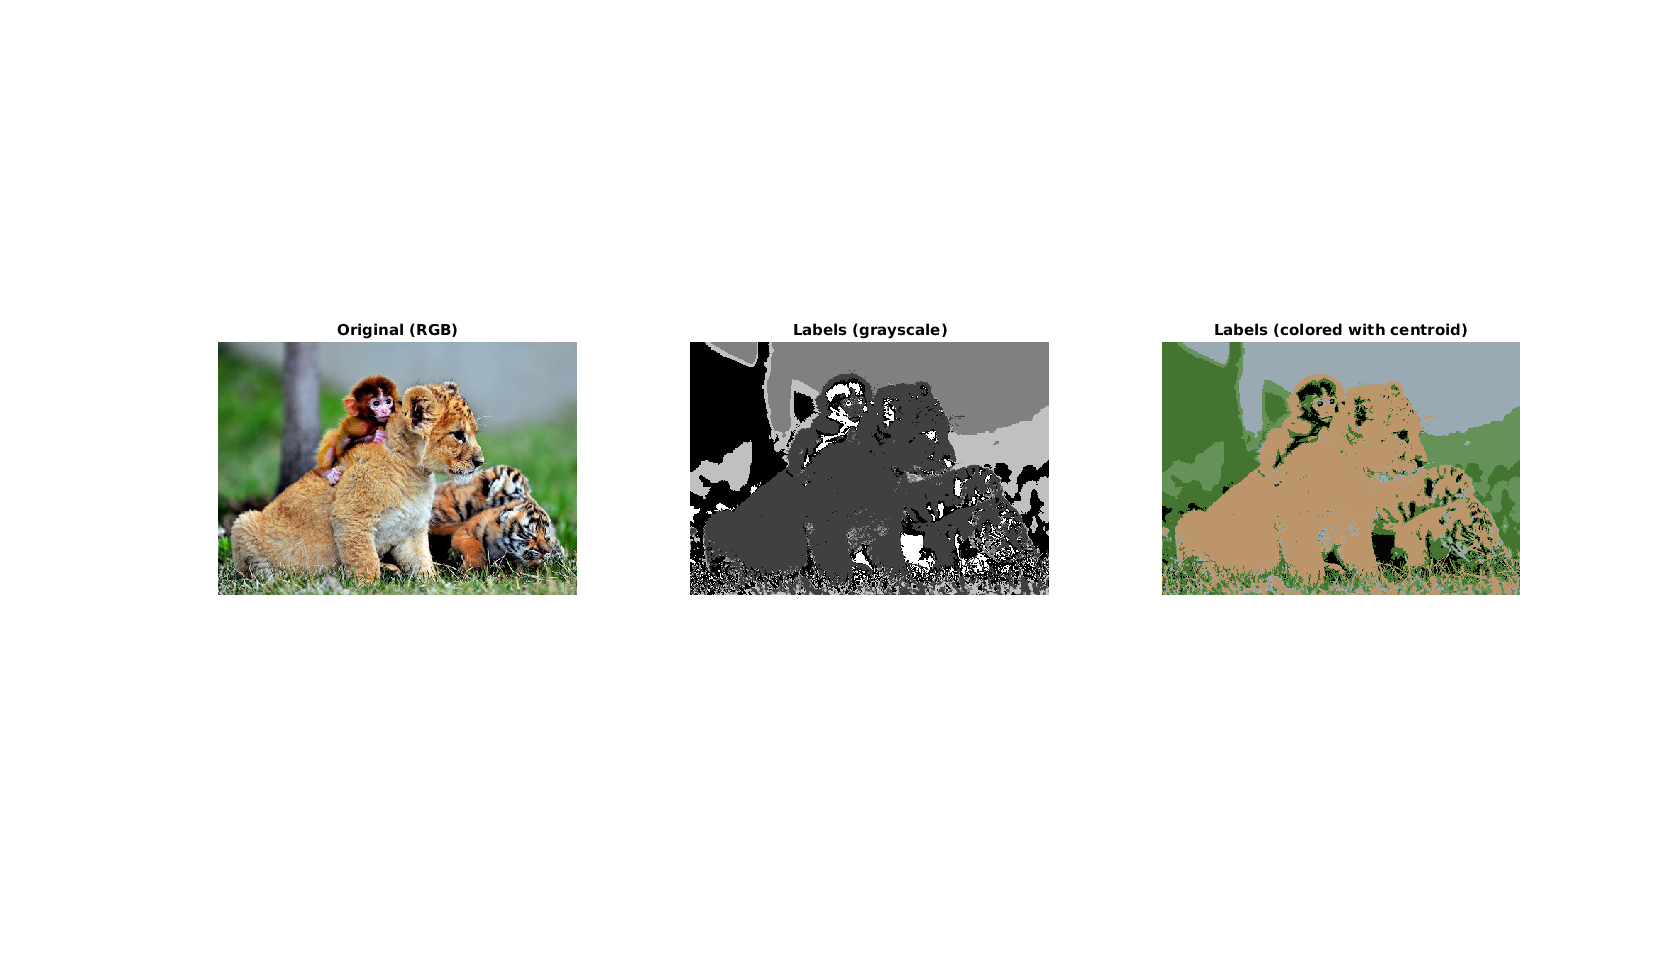
\includegraphics[trim={50px 250px 50px 220px},clip,width=\textwidth]{img/mshift/animals_d30_no_spatial.png}
\caption{Segmentation of \texttt{animals.jpg} with Mean-shift}
\label{fig:animals-d30-no-spatial}
\end{figure}

Other examples of segmentation with Mean-shift are shown in figures
\ref{fig:alwin2-d30-no-spatial} and in \ref{fig:bigbangfamily-d30-no-spatial}.
We can appreciate a good segmentation quality in general. There are some
effects that could possibly be avoided with a lower bandwidth, like some
pieces of clothing being assigned to the same cluster as the skin and
the cheeks of the squirrels being assigned to the same cluster as the background.

\begin{figure}[hbt]
\centering
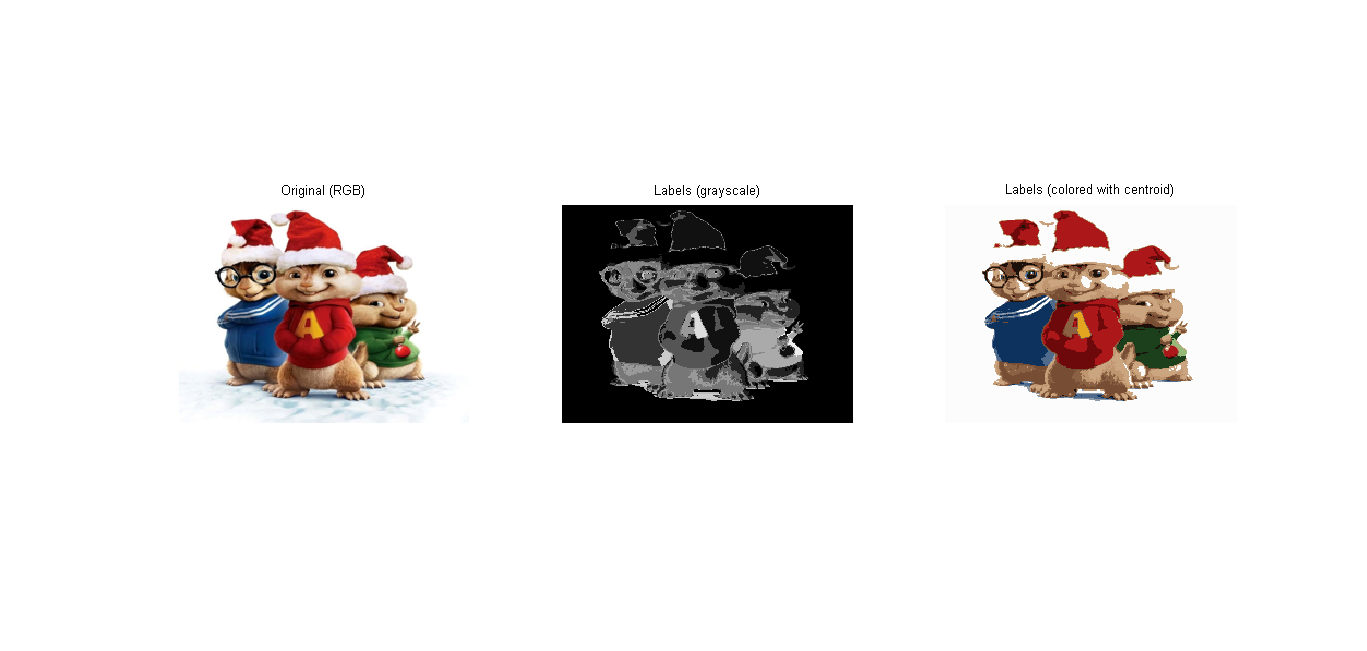
\includegraphics[trim={50px 100px 50px 100px},clip,width=\textwidth]{img/mshift/alwin2_d30_no_spatial.png}
\caption{Segmentation of \texttt{alwin2.jpg} with Mean-shift}
\label{fig:alwin2-d30-no-spatial}
\end{figure}

\begin{figure}[hbt]
\centering
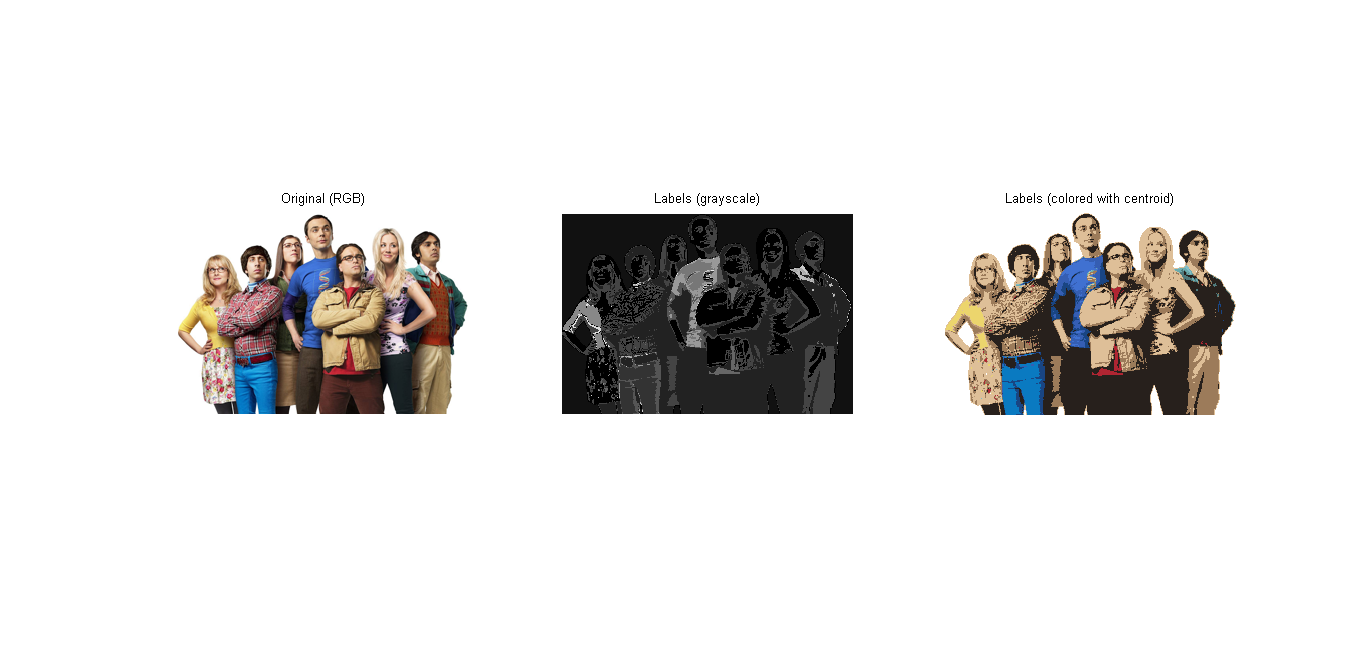
\includegraphics[trim={50px 100px 50px 100px},clip,width=\textwidth]{img/mshift/bigbang_d30_no_spatial.png}
\caption{Segmentation of \texttt{bigbangfamily.png} with Mean-shift}
\label{fig:bigbangfamily-d30-no-spatial}
\end{figure}

The algorithm is not deterministic because at each update step the next
point to update (i.e. move towards the center of mass of its neighbourhood)
is selected randomly. This is done in the 
line 47 of the provided \texttt{MeanShiftCluster.m} file
(\texttt{tempInd = ceil( (numInitPts-1e-6)*rand);}).
This also means that two executions of the Mean-shift algorithm do
not yield necessarily the same value
(unless the seed of the random generator is fixed). This can be
observed in figure \ref{fig:animals-d30-differences}

\begin{figure}[hbt]
\centering
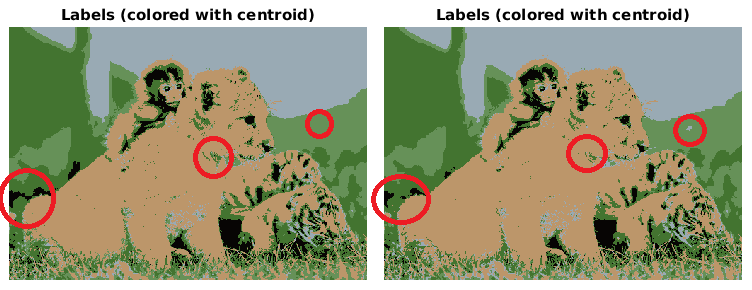
\includegraphics[width=\textwidth]{img/mshift/animals_d30_differences.png}
\caption[Results of two successive runs of Mean-shift]{Results of two successive runs of Mean-shift. The most noticeable differences are marked with a red circle.}
\label{fig:animals-d30-differences}
\end{figure}

Much like with k-means, geometric transformations lead to different results.
This is observed in figures \ref{fig:animals-d30-no-spatial-scaled-down} and
\ref{fig:animals-d30-no-spatial-rotated}, because
the order in which the active points are picked to be shifted is dependent on the
structure of the data passed to the algorithm.

\begin{figure}[hbt]
\centering
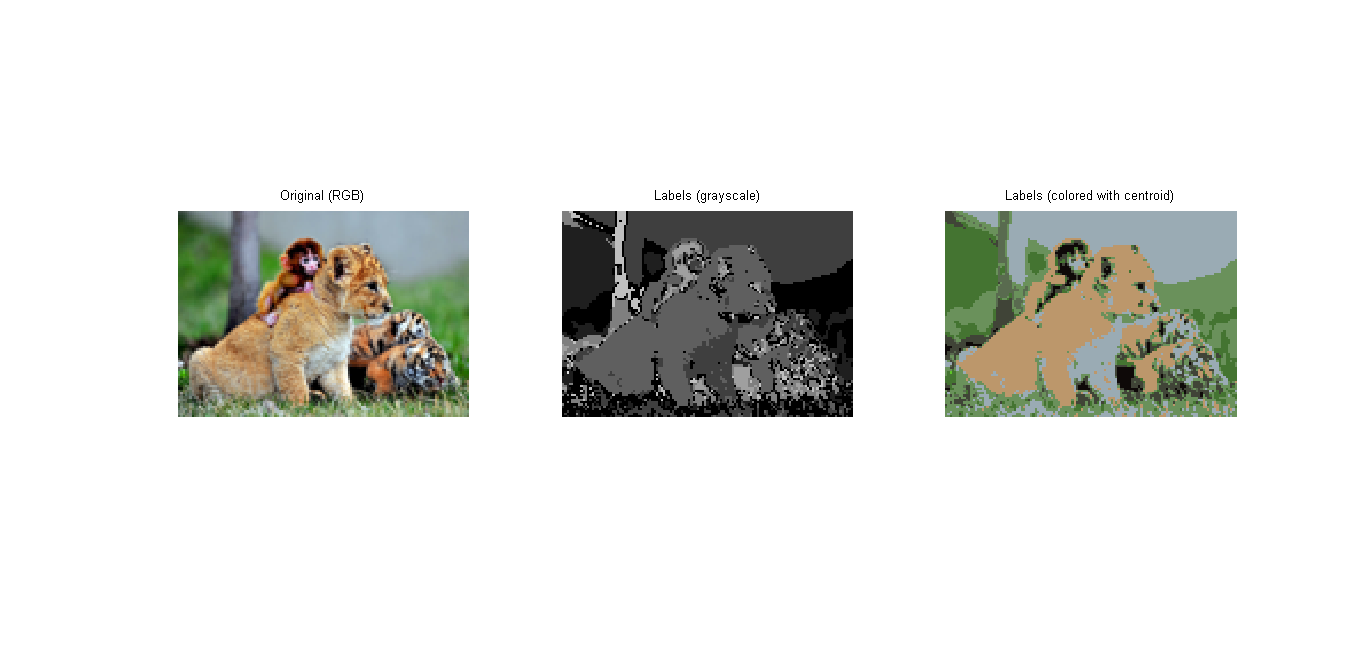
\includegraphics[trim={50px 100px 50px 100px},clip,width=\textwidth]{img/mshift/animals_d30_no_spatial_scaled_down.png}
\caption{Segmentation of \texttt{animals.jpg} (scaled down, s=0.25) with Mean-shift}
\label{fig:animals-d30-no-spatial-scaled-down}
\end{figure}

\begin{figure}[hbt]
\centering
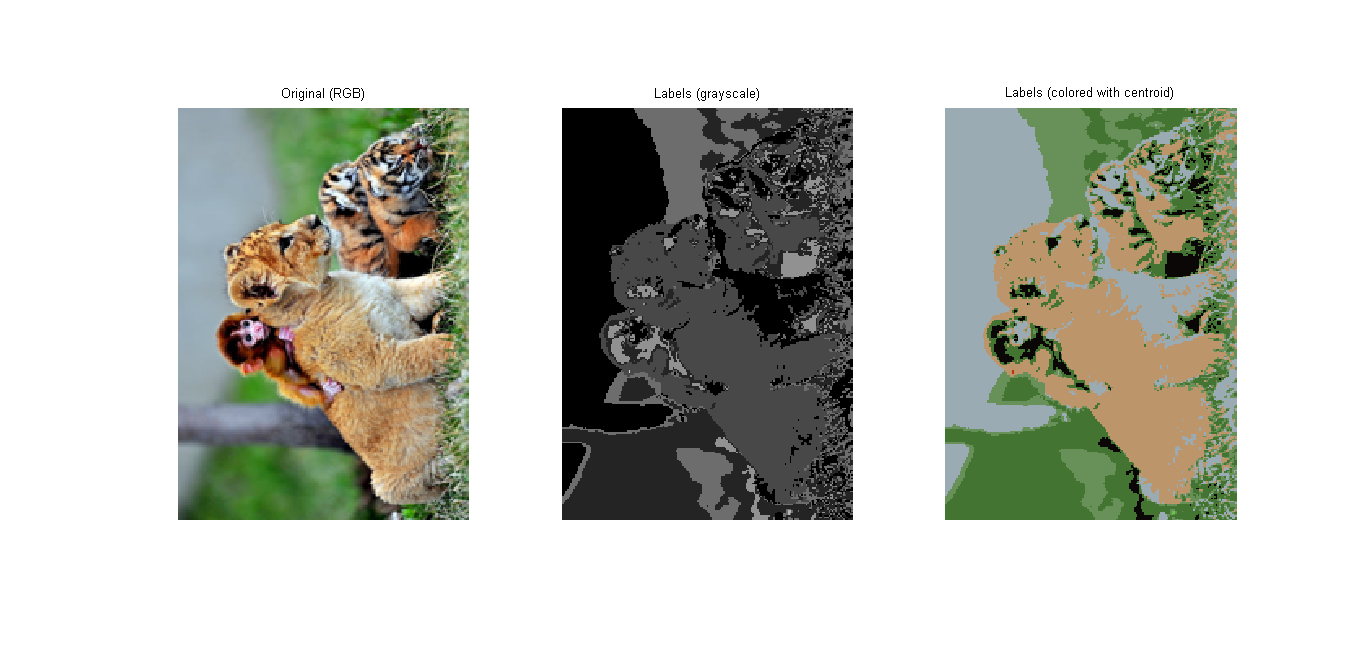
\includegraphics[trim={50px 100px 50px 100px},clip,width=\textwidth]{img/mshift/animals_d30_no_spatial_scaled_down_rotated.png}
\caption{Segmentation of \texttt{animals.jpg} (rotated) with Mean-shift}
\label{fig:animals-d30-no-spatial-rotated}
\end{figure}

It is also interesting to observe the effect of the bandwidth on the segmentation.
We expect that a high bandwidth leads to grouping more active points in the same
cluster, reducing the total number of clusters. On the other hand a higher bandwidth
helps to reduce the number of active points earlier in the algorithm, which means
that the runtime is lower. Therefore the bandwidth should be increased either to
fight over-segmentation problems. To illustrate this explanation we provide figure
\ref{fig:bigbangfamily-d50-no-spatial} which shows a result generated with a
bandwidth of 50 and has less clusters than the segmentation showed in figure
\ref{fig:bigbangfamily-d30-no-spatial}. Figure \ref{fig:animals-d50-no-spatial} is another
example that in addition shows how the bandwidth can be used to produce a somewhat less noisy
segmentation (compare it to figure \ref{fig:animals-d30-no-spatial}).

\begin{figure}[hbt]
\centering
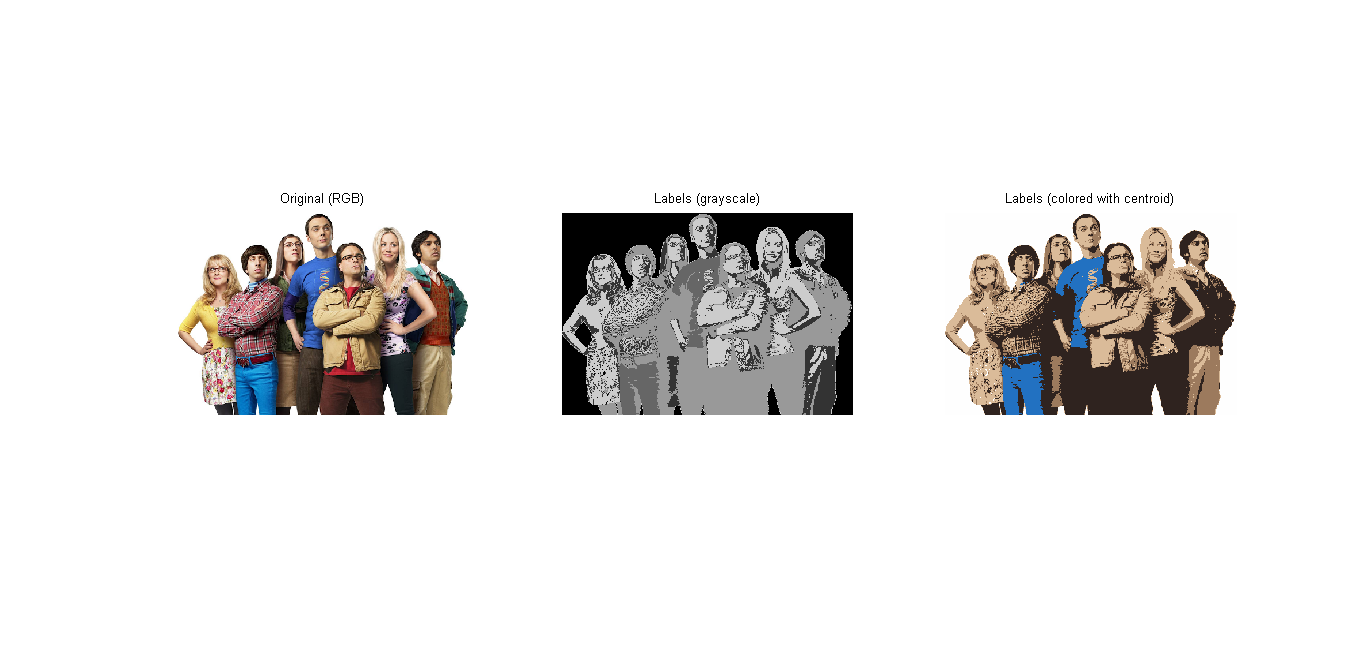
\includegraphics[trim={50px 100px 50px 100px},clip,width=\textwidth]{img/mshift/bigbang_d50_no_spatial.png}
\caption{Segmentation of \texttt{bigbangfamily.png} with Mean-shift. BW = 50}
\label{fig:bigbangfamily-d50-no-spatial}
\end{figure}

\begin{figure}[hbt]
\centering
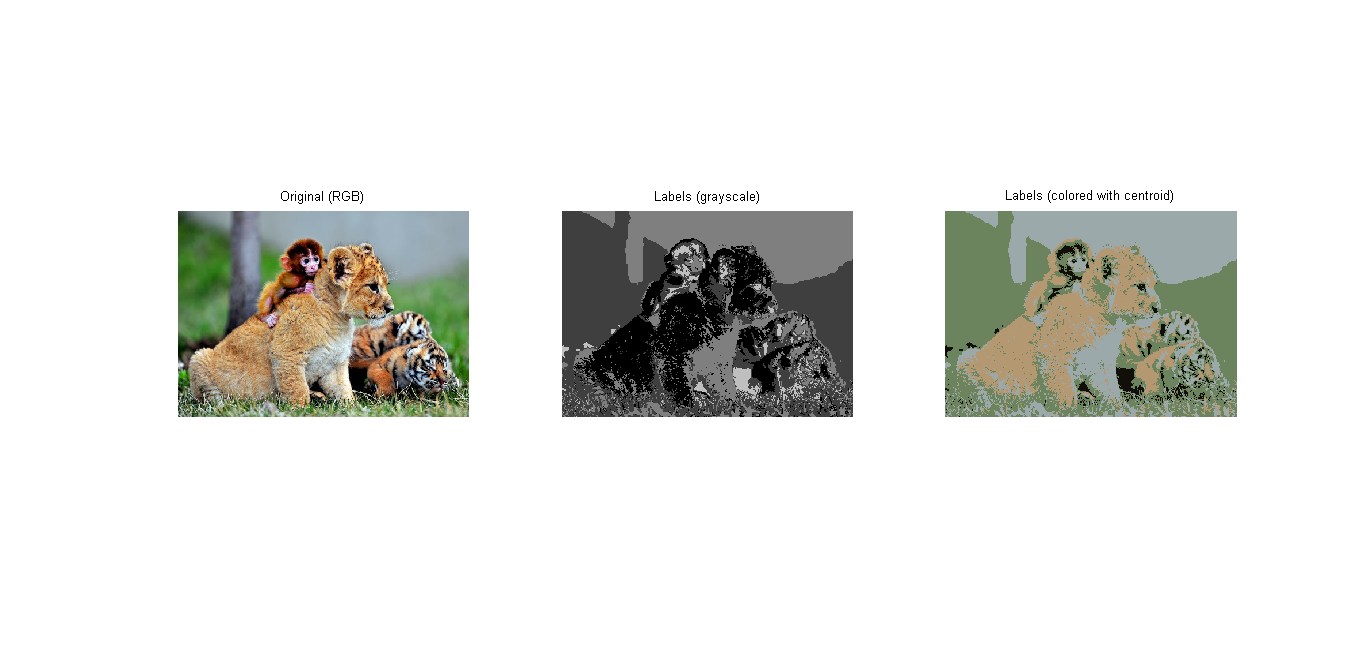
\includegraphics[trim={50px 100px 50px 100px},clip,width=\textwidth]{img/mshift/animals_d50_no_spatial.png}
\caption{Segmentation of \texttt{animals.jpg} with Mean-shift. BW = 50}
\label{fig:animals-d50-no-spatial}
\end{figure}

\FloatBarrier

\subsection{Adding spatial information to the Mean-shift segmentation}

Finally we discuss the effect of adding spatial information to the data passed to the
Mean-shift algorithm. In figure \ref{fig:animals-d30-spatial} we can see the
\texttt{animals.jpg} scaled down image segmented with spatial coordinates and a bandwidth of
30 (for this section we will used either scaled down images or high bandwidths in order
to produce results in a reasonable amount of time). Much like in k-means, the effect of
considering the spatial coordinates is obtaining smoother regions but with the possibility
of dividing large objects. More examples are shown in figures \ref{fig:alwin2-d30-spatial} and
\ref{fig:bigbangfamily-d30-spatial}. The lion
of figure \ref{fig:animals-d50-spatial} is a particularly good example of how a big entity
is cut asunder into several regions.

\begin{figure}[hbt]
\centering
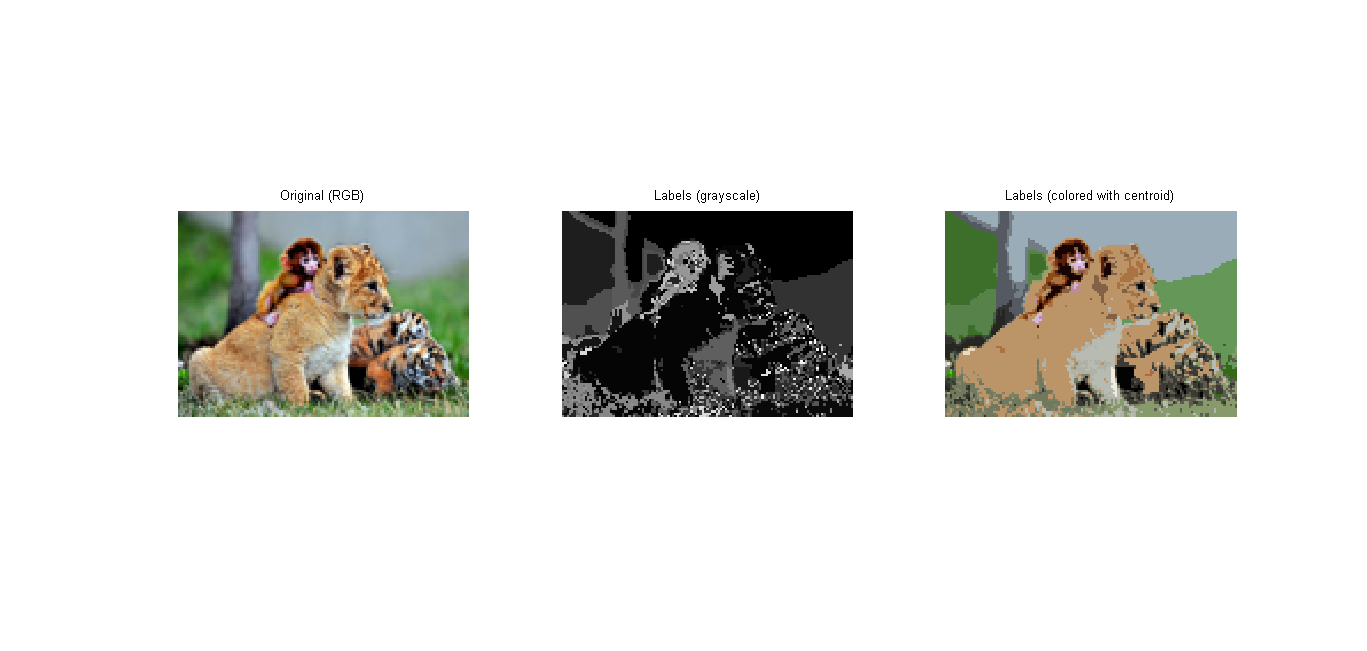
\includegraphics[trim={50px 100px 50px 100px},clip,width=\textwidth]{img/mshift/animals_d30_spatial_scaled_down.png}
\caption{Segmentation of scaled down (s=0.5) \texttt{animals.jpg} with Mean-shift and spatial information.}
\label{fig:animals-d30-spatial}
\end{figure}

\begin{figure}[hbt]
\centering
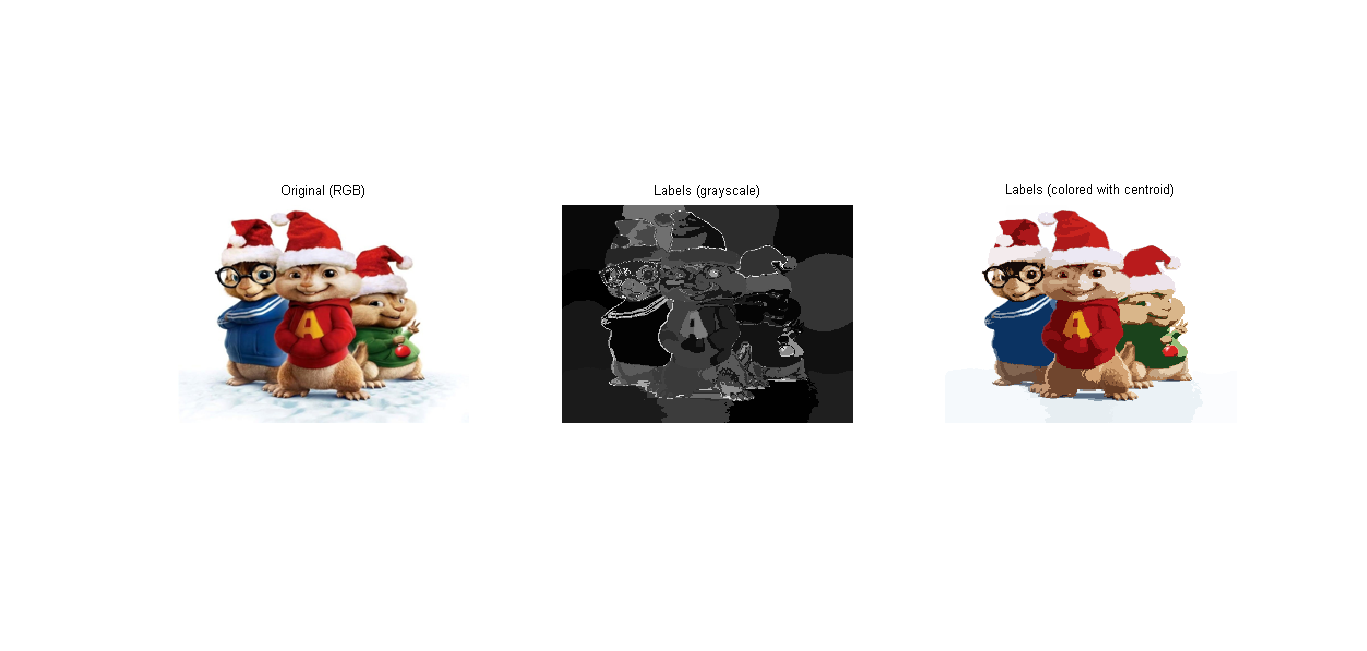
\includegraphics[trim={50px 100px 50px 100px},clip,width=\textwidth]{img/mshift/alwin2_d30_spatial.png}
\caption{Segmentation of scaled down (s=0.25) \texttt{alwin2.jpg} with Mean-shift and spatial information.}
\label{fig:alwin2-d30-spatial}
\end{figure}

\begin{figure}[hbt]
\centering
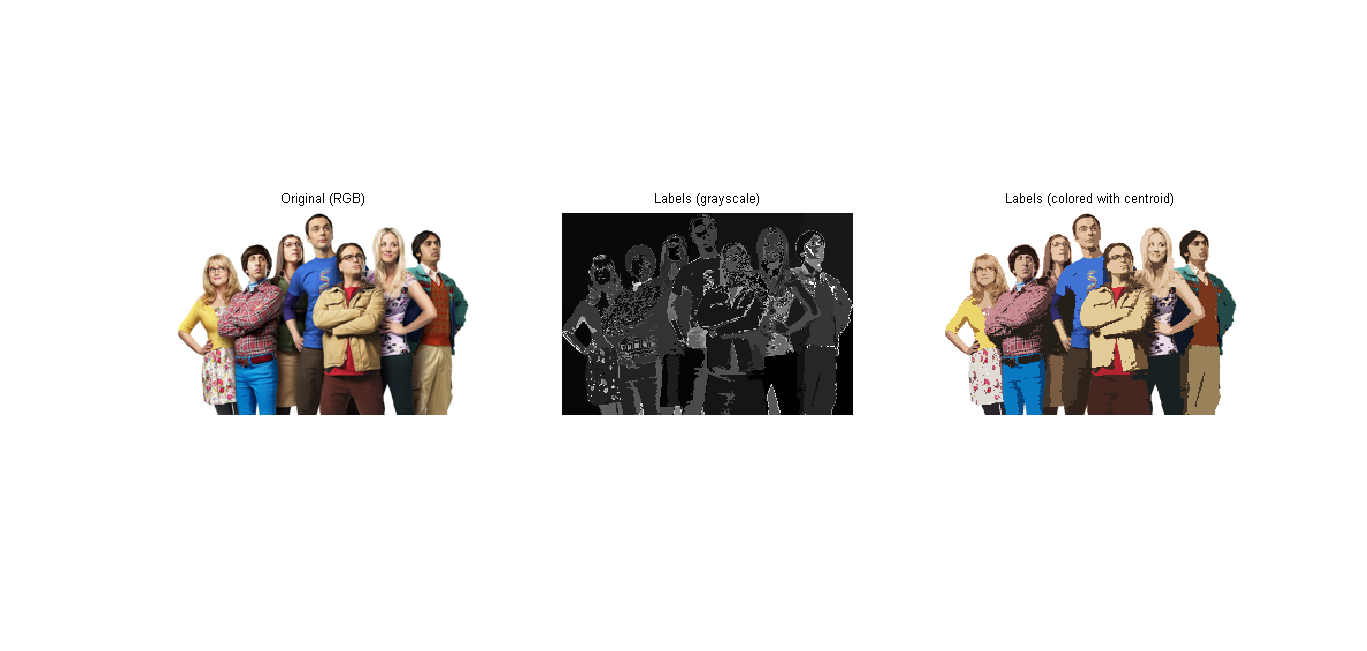
\includegraphics[trim={50px 100px 50px 100px},clip,width=\textwidth]{img/mshift/bigbang_d30_spatial_scaled_down.png}
\caption{Segmentation of scaled down (s=0.5) \texttt{bigbangfamily.png} with Mean-shift and spatial information.}
\label{fig:bigbangfamily-d30-spatial}
\end{figure}

\begin{figure}[hbt]
\centering
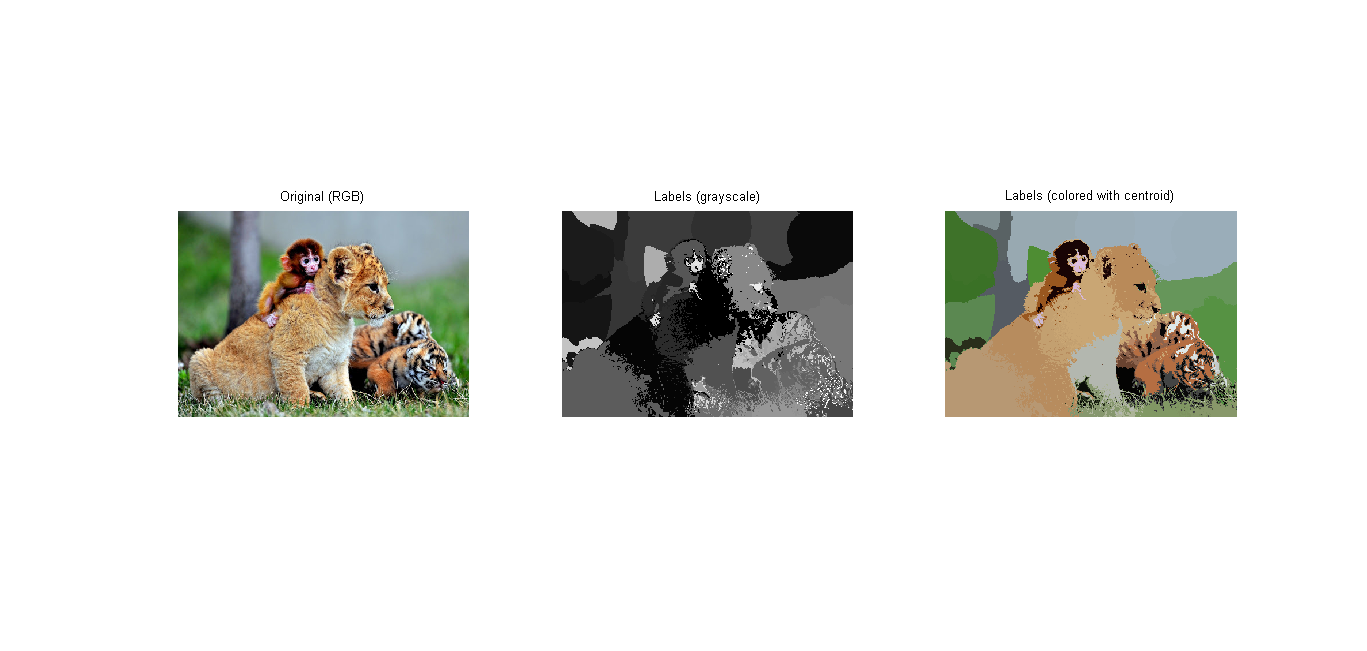
\includegraphics[trim={50px 100px 50px 100px},clip,width=\textwidth]{img/mshift/animals_d50_spatial.png}
\caption{Segmentation of full-size \texttt{animals.jpg} with Mean-shift and spatial information. BW=50}
\label{fig:animals-d50-spatial}
\end{figure}